\chapter{Analisis}
\label{chap:analisis}
Bab ini berisi analisis yang digunakan pada skripsi ini, analisis hasil survei perekaman kehadiran daring dan luring, analisis alur perekaman kehadiran online, cara menerjemahkan perekaman kehadiran online ke dalam selenium, dan analisis program sejenis.

\section{Analisis Hasil Survei Perekaman Kehadiran Daring dan Luring}
\label{sec:survei} 
Berdasarkan hasil survei yang telah diterima dari 21 orang responden yang merupakan mahasiswa Teknik Informatika Universitas Katolik
Parahyangan yang terdiri dari mahasiswa angkatan 2017 sampai 2019, dengan pertanyaan yang diajukan kepada responen dan rangkuman jawaban hasil survei sebagai berikut:
\begin{enumerate}
	\item \textbf{Berapa detik perkiraan waktu interaksi yang Anda butuhkan untuk melakukan perekaman kehadiran daring di \url{https://studentportal.unpar.ac.id/}, mulai dari membuka \textit{browser}, lalu masuk ke \url{https://studentportal.unpar.ac.id/}, lalu mengklik tombol presensi?}\\
	Jawaban dari 21 orang responden adalah mulai dari waktu paling cepat 10 detik hingga waktu paling lama 600 detik.\\ \\
	 \begin{tabular}{|p{4cm} |p{7cm}|}
		\hline
		Jumlah Responden &  Waktu Perekaman Kehadiran Daring \\ \hline     
		1 orang &  10 detik\\ \hline 
		1 orang &  13 detik\\ \hline 
		5 orang &  15 detik\\ \hline 
		2 orang &  17 detik\\ \hline 
		2 orang &  18 detik\\ \hline 
		3 orang &  20 detik\\ \hline
		1 orang &  25 detik\\ \hline 
		1 orang &  30 detik\\ \hline 
		2 orang &  45 detik\\ \hline
		1 orang &  50 detik\\ \hline 
		1 orang &  300 detik\\ \hline 
		1 orang &  600 detik\\ \hline
	\end{tabular}\\ \\
	Jika dihitung rata-rata waktu yang dibutuhkan untuk melakukan perekaman kehadiran daring bagi para mahasiswa adalah 63 detik.
	
	\item \textbf{Berapa detik perkiraan waktu interaksi yang Anda butuhkan untuk melakukan perekaman kehadiran luring menggunakan metode tanda tangan seperti pembelajaran di kelas, mulai dari mengambil kertas absen, lalu tanda tangan, lalu memberikannya ke rekan di sebelah anda?}\\
	Jawaban dari 21 orang responden adalah mulai dari waktu paling cepat 5 detik hingga waktu paling lama 15 detik.\\ \\
	  \begin{tabular}{|p{4cm} |p{7cm}|}
		\hline
		Jumlah Responden &  Waktu Perekaman Kehadiran Luring \\ \hline     
		5 orang &  5 detik\\ \hline 
		1 orang &  6 detik\\ \hline 
		5 orang &  7 detik\\ \hline 
		2 orang &  8 detik\\ \hline 
		7 orang &  10 detik\\ \hline 
		1 orang &  15 detik\\ \hline
	\end{tabular}\\ \\
	Jika dihitung rata-rata waktu yang dibutuhkan untuk melakukan perekaman kehadiran luring bagi para mahasiswa adalah 7,95 detik.
\end{enumerate}
Sedangkan hasil survei yang telah diterima dari 6 orang responden yang merupakan dosen Teknik Informatika Universitas Katolik Parahyangan, dengan pertanyaan yang diajukan kepada responen dan rangkumana jawaban hasil survei sebagai berikut:
\begin{enumerate}
	\item \textbf{Berapa detik perkiraan waktu interaksi yang Anda butuhkan untuk melakukan perekaman kehadiran daring di \url{https://akuhadir.unpar.ac.id} ?}\\
	Jawaban dari 6 orang responden adalah mulai dari waktu paling cepat 1 detik hingga waktu paling lama 120 detik.\\ \\
	\begin{tabular}{|p{4cm} |p{7cm}|}
		\hline
		Jumlah Responden &  Waktu Perekaman Kehadiran Daring \\ \hline     
		1 orang &  1 detik\\ \hline 
		1 orang &  10 detik\\ \hline 
		2 orang &  15 detik\\ \hline 
		1 orang &  30 detik\\ \hline 
		1 orang &  120 detik\\ \hline 
	\end{tabular}\\ \\
	Jika dihitung rata-rata waktu yang dibutuhkan untuk melakukan perekaman kehadiran daring bagi para dosen adalah 31,83 detik.
	
	\item \textbf{Berapa detik perkiraan waktu interaksi yang Anda butuhkan untuk melakukan perekaman kehadiran luring menggunakan metode fingerprint?}\\
	Jawaban dari 6 orang responden adalah mulai dari waktu paling cepat 1 detik hingga waktu paling lama 90 detik.\\ \\
	\begin{tabular}{|p{4cm} |p{7cm}|}
		\hline
		Jumlah Responden &  Waktu Perekaman Kehadiran Luring \\ \hline     
		1 orang &  1 detik\\ \hline 
		3 orang &  5 detik\\ \hline 
		1 orang &  40 detik\\ \hline 
		1 orang &  90 detik\\ \hline 
	\end{tabular}\\ \\
	Jika dihitung rata-rata waktu yang dibutuhkan untuk melakukan perekaman kehadiran luring bagi para dosen adalah 24,33 detik.
\end{enumerate}
	Hasil survei tersebut menunjukan bahwa waktu yang dibutuhkan untuk perekaman kehadiran secara luring lebih cepat bagi para mahasiswa maupun dosen dibandingkan waktu yang dibutuhkan untuk perekaman kehadiran secara daring. 

\section{Analisis Alur Perekaman Kehadiran Online}
\label{sec:alur} 
Portal Akademik Mahasiswa Universitas Katolik Parahyangan yang terbaru sejak 2020 sudah dapat melakukan perekaman kehadiran secara online untuk setiap mata kuliah yang diambil. Berikut ini adalah alur untuk melakukan perekaman kehadiran online melalui Portal Akademik Mahasiswa Universitas Katolik Parahyangan:
\begin{enumerate}
	\item Melakukan akses Portal Akademik Mahasiswa yang dapat diakses melalui \url{https://studentportal.unpar.ac.id/}.
	\begin{figure}[H]
		\centering
		
\includegraphics[scale=0.225]{Gambar/halaman2019.jpg}
		\caption{Tampilan halaman awal Portal Akademik Mahasiswa} 
		\label{fig:studpor_home_2019}
	\end{figure}
	\item Menekan tombol ``Login'' yang sudah tersedia agar dapat masuk ke dalam Portal Akademik Mahasiswa, dapat dilihat pada Gambar \ref{fig:studpor_home_2019}.
	
	\item Memasukan \textit{email} mahasiswa.
	\begin{figure}[H]
		\centering
		
\includegraphics[scale=0.225]{Gambar/login.jpg}
		\caption{Tampilan halaman Portal Akademik Mahasiswa untuk memasukan \textit{email}} 
		\label{fig:login}
	\end{figure}
	\item Menekan tombol ``NEXT'' setelah memasukan \textit{email}, dapat dilihat pada Gambar \ref{fig:login}.
	
	\item Memasukan \textit{password} milik mahasiswa.
	\begin{figure}[H]
		\centering
		
\includegraphics[scale=0.225]{Gambar/pass.jpg}
		\caption{Tampilan halaman Portal Akademik Mahasiswa untuk memasukan \textit{password}} 
		\label{fig:pass}
	\end{figure}
	\item Menekan tombol ``LOGIN'' setelah memasukan \textit{password}, dapat dilihat pada Gambar \ref{fig:pass}.
	
	\item Menekan tombol ``Tutup'' jika muncul peringatan atau langsung menekan tombol berbentuk heksagon ``JADWAL \& KEHADIRAN'' jika tidak muncul peringatan.
	\begin{figure}[H]
		\centering
		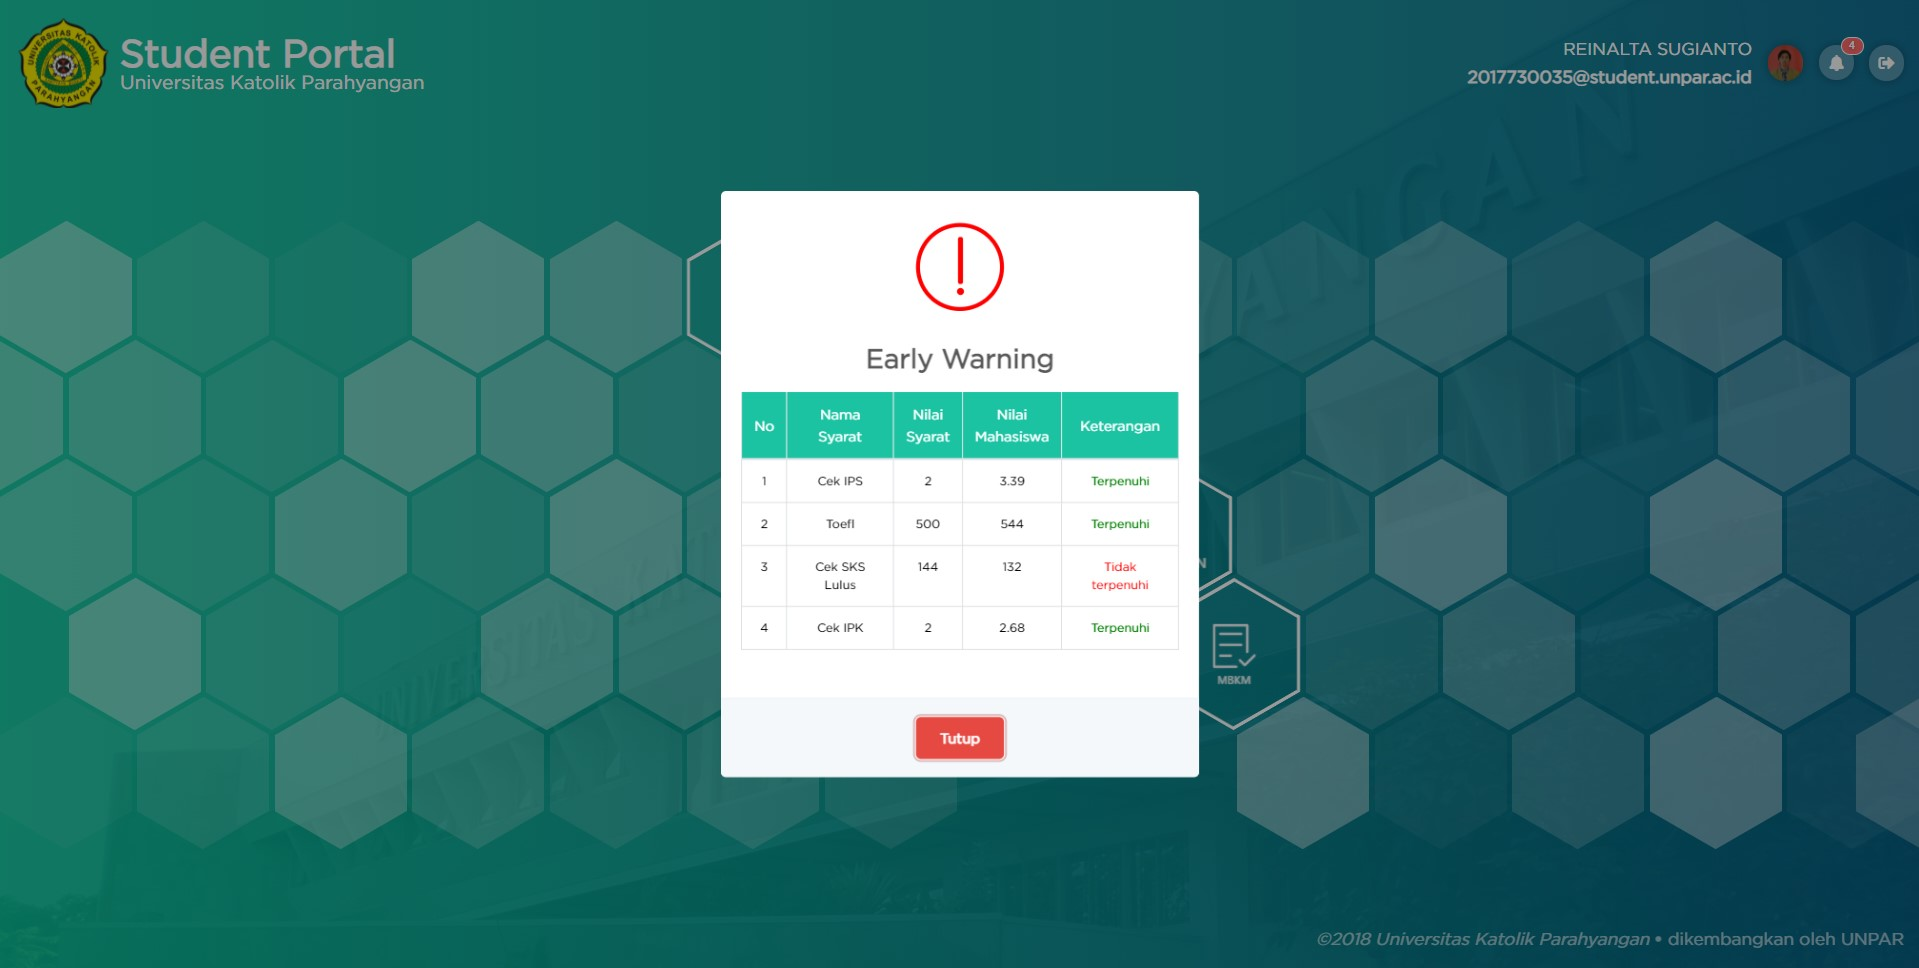
\includegraphics[scale=0.225]{Gambar/notif.jpg}
		\caption{Tampilan peringatan pada halaman Portal Akademik Mahasiswa} 
		\label{fig:notif}
	\end{figure}

	\begin{figure}[H]
		\centering
		
\includegraphics[scale=0.225]{Gambar/jadwal.jpg}
		\caption{Tampilan halaman Portal Akademik Mahasiswa setelah Berhasil \textit{Login}} 
		\label{fig:jadwal}
	\end{figure}
	Pada Gambar \ref{fig:notif} merupakan sebuah peringatan yang terkadang muncul menjelang berakhirnya suatu semester untuk melihat status kebutuhan mahasiswa untuk lulus, sehingga perlu menekan tombol ``Tutup'' terlebih dahulu untuk menekan tombol berbentuk heksagon ``JADWAL \& KEHADIRAN'' seperti pada Gambar \ref{fig:jadwal}. Jika tidak terjadi peringatan seperti pada  Gambar \ref{fig:notif}, maka dapat langsung menekan tombol berbentuk heksagon ``JADWAL \& KEHADIRAN'' seperti pada Gambar \ref{fig:jadwal}.
	
	\item Menekan tombol berwarna merah pada kolom bagian persensi dari tabel jadwal kehadiran mata kuliah. 
	\begin{figure}[H]
		\centering
		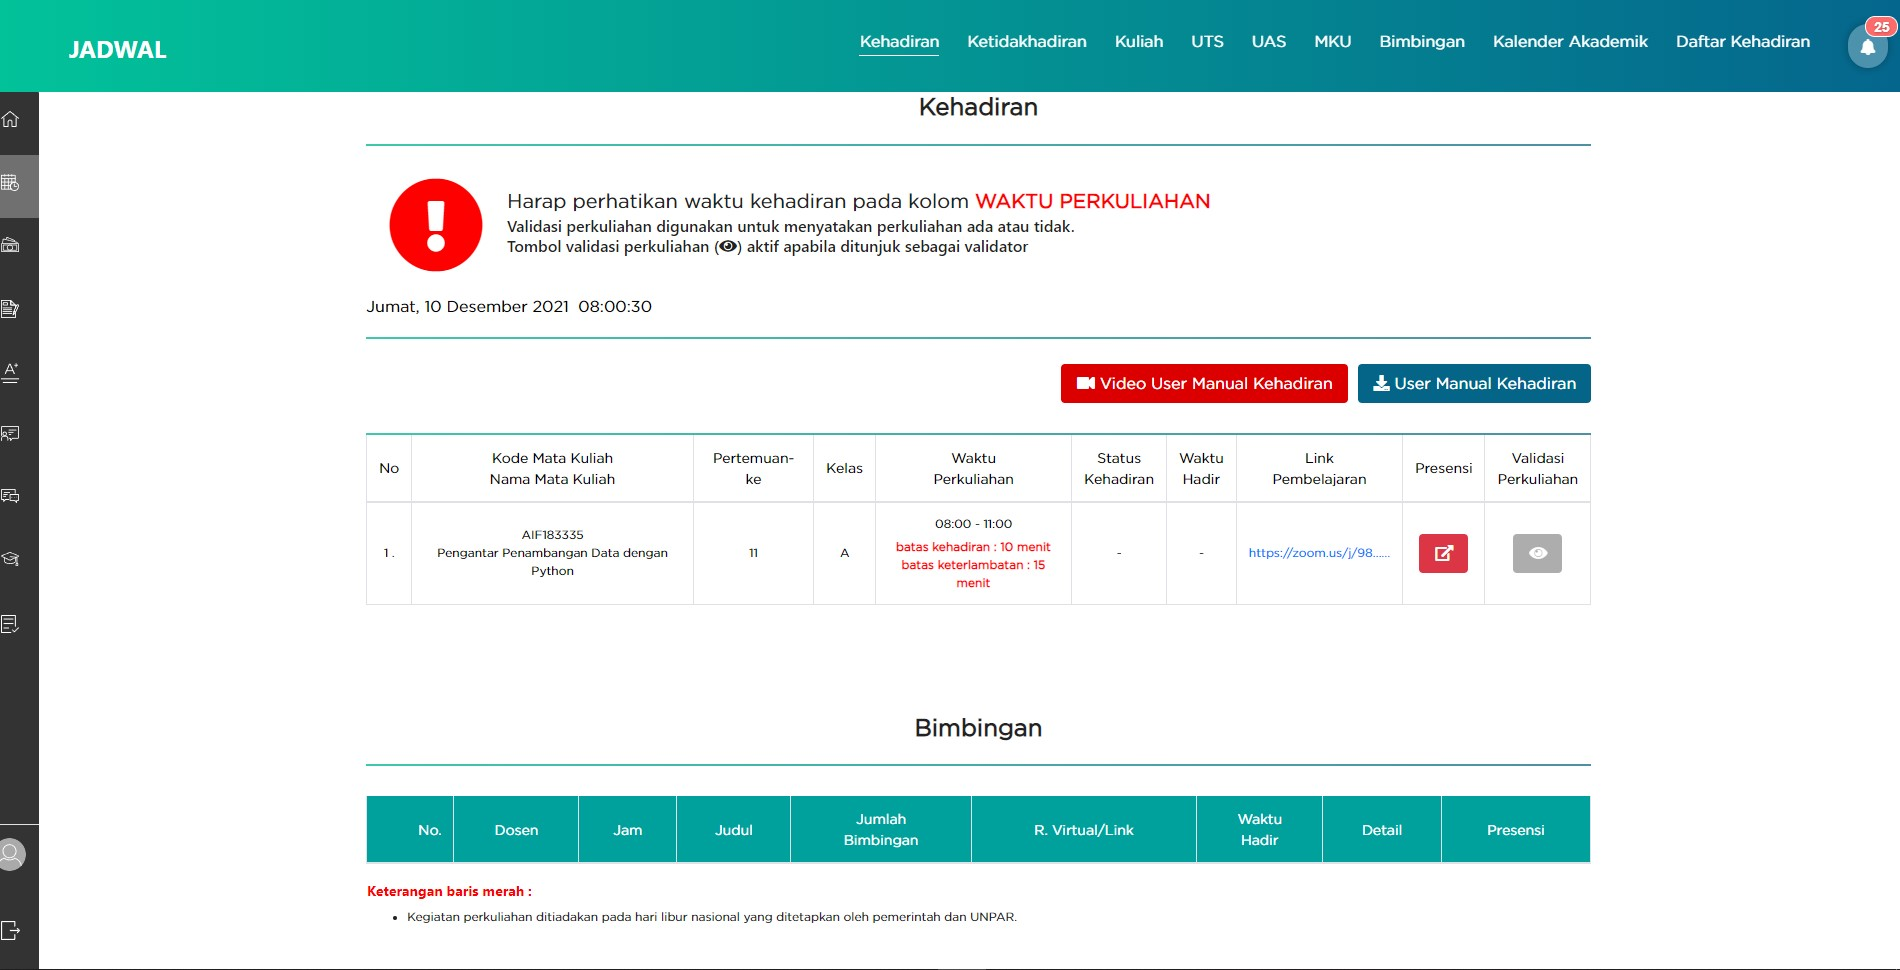
\includegraphics[scale=0.225]{Gambar/absen.jpg}
		\caption{Tampilan halaman Portal Akademik Mahasiswa untuk Melakukan Absen} 
		\label{fig:absen}
	\end{figure}

	\item Menekan tombol ``OK'' ketika muncul pemberitahuan setelah berhasil melakukan presensi.
	\begin{figure}[H]
		\centering
		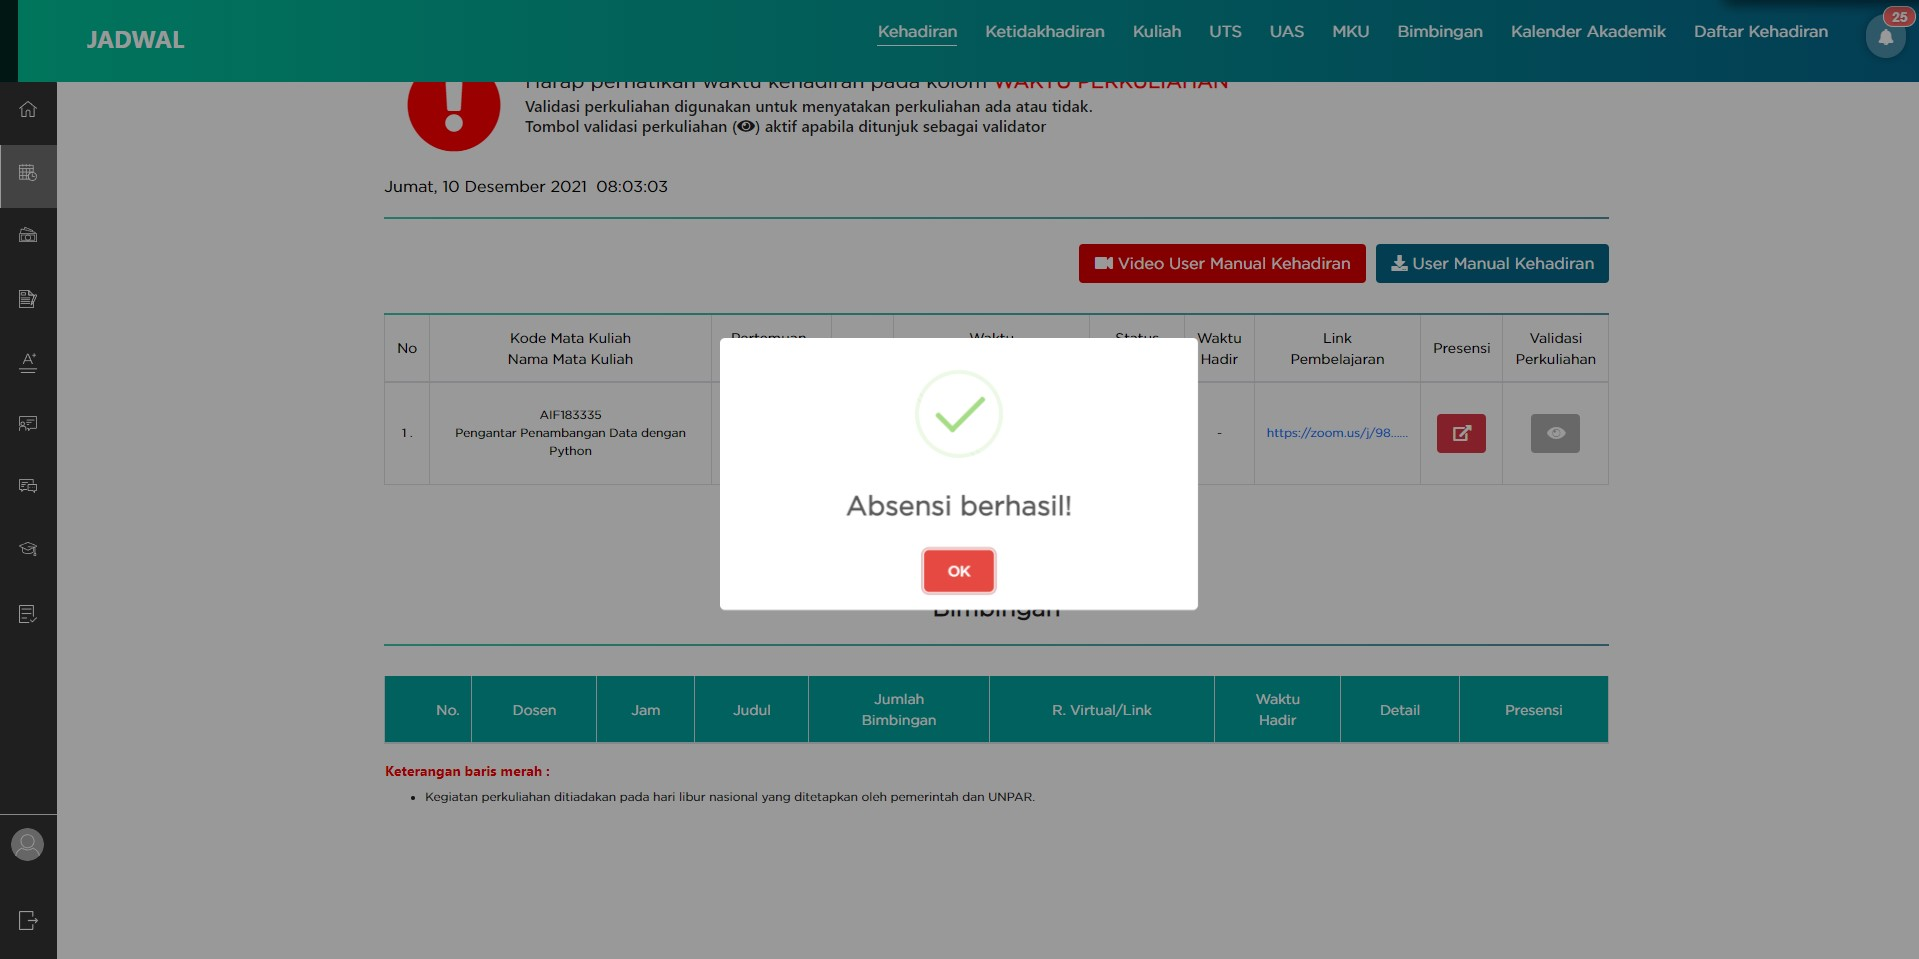
\includegraphics[scale=0.225]{Gambar/berhasilAbsen.jpg}
		\caption{Tampilan Pemberitahuan Absensi Berhasil} 
		\label{fig:berhasil}
	\end{figure}
\end{enumerate}

\section{Cara Menerjemahkan Perekaman Kehadiran Online ke dalam Selenium}
\label{sec:terjemah} 
Otomatisasi perekaman kehadiran online ini akan menggunakan selenium, sehingga perlu diterjemahkan dari cara perekaman kehadiran online secara normal ke dalam selenium. Membuka situs web \url{https://studentportal.unpar.ac.id/} menggunakan selenium adalah dengan menggunakan \textit{method get()}. Setiap tombol yang ingin ditekan akan diambil elemennya agar dapat diotomatisasikan dengan selenium. Pada \textit{browser} Google Chrome, cara mendapatkan setiap elemen yang dibutuhkan adalah dengan melakukan \textit{inspect} elemen pada bagian yang ingin diambil elemennya. Elemen yang ingin diambil dapat dilakukan dengan berbagai macam cara seperti yang sudah dijelaskan pada Bab \ref{sec:selenium}, namun yang utama akan dipilih adalah dengan mengambil elemen berdasarkan \textit{CSS selector}, tetapi tidak menutup kemungkinan menggunakan cara yang lain untuk menemukan suatu elemen. Jika mengambil elemen berdasarkan \textit{CSS selector} tidak perlu takut jika struktur HTML atau nama elemen diubah, karena \textit{CSS selector} sangat jarang diubah saat melakukan pembaharuan pada suatu situs web. Dalam melakukan otomatisasi perekaman kehadiran online pasti perlu memasukan \textit{email} dan \textit{password}, untuk memasukan hal tersebut perlu menggunakan \textit{method sendKeys()}. Memasukan \textit{email} dan \textit{password} ini tidak langsung dimasukan ke dalam programnya, akan tetapi melalui file konfigurasi yang diisi \textit{email} dan \textit{password}, lalu dipanggil ke kode programnya. 

\section{Analisis Program Sejenis}
\label{sec:seleniumIDE}  
Selenium IDE merupakan program \textit{open source} untuk otomatisasi di web. Selenium IDE dapat di \textit{install} di browser, contohnya di Google Chrome yang setelah di \textit{install} akan menjadi \textit{extensions}. \textit{Extensions} di Google Chrome adalah sebuah aplikasi kecil yang dapat dijalankan pada Google Chrome itu sendiri. Berikut ini langkah-langkah untuk melakukan otomatisasi menggunakan Selenium IDE:
	\begin{enumerate}
		\item Membuka Selenium Ide yang tersimpan di \textit{Extensions} pada Google Chrome.
		\item Memilih menu \textit{Record a new test in a new project} (merekam tes baru untuk proyek baru).
		\begin{figure}[H]
			\centering
			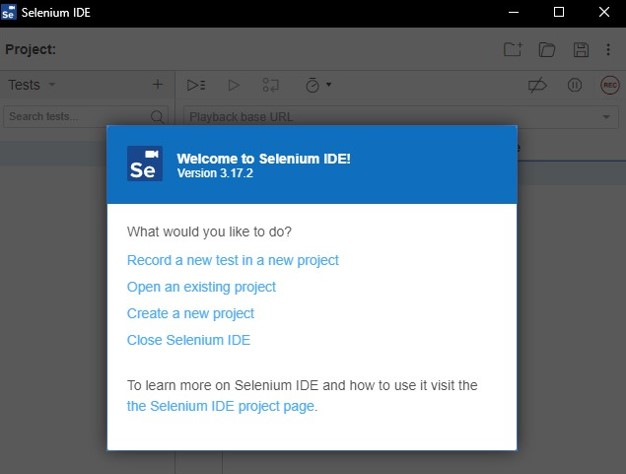
\includegraphics[scale=0.4]{Gambar/menuSeleniumIDE.jpg}
			\caption{Tampilan Menu Awal Selenium IDE} 
			\label{fig:menuSeleniumIDE}
		\end{figure}
		\item Memasukan nama proyek, lalu tekan tombol ``OK''. 
		\begin{figure}[H]
			\centering
			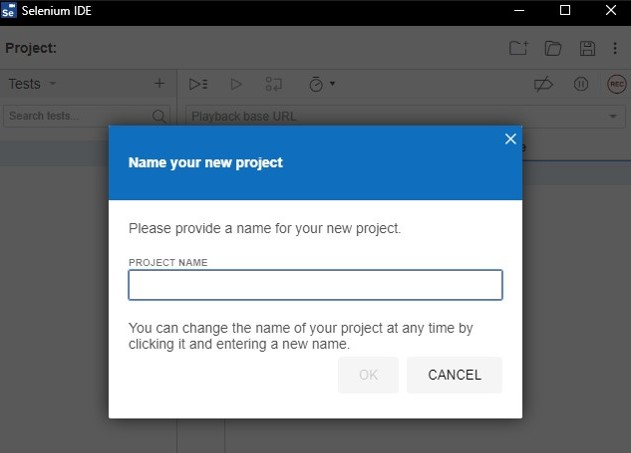
\includegraphics[scale=0.4]{Gambar/namaProyek.jpg}
			\caption{Tampilan Memasukan Nama Proyek} 
			\label{fig:namaProyek}
		\end{figure}
		\item Memasukan situs web, lalu menekan tombol ``START RECORDING''
		\begin{figure}[H]
			\centering
			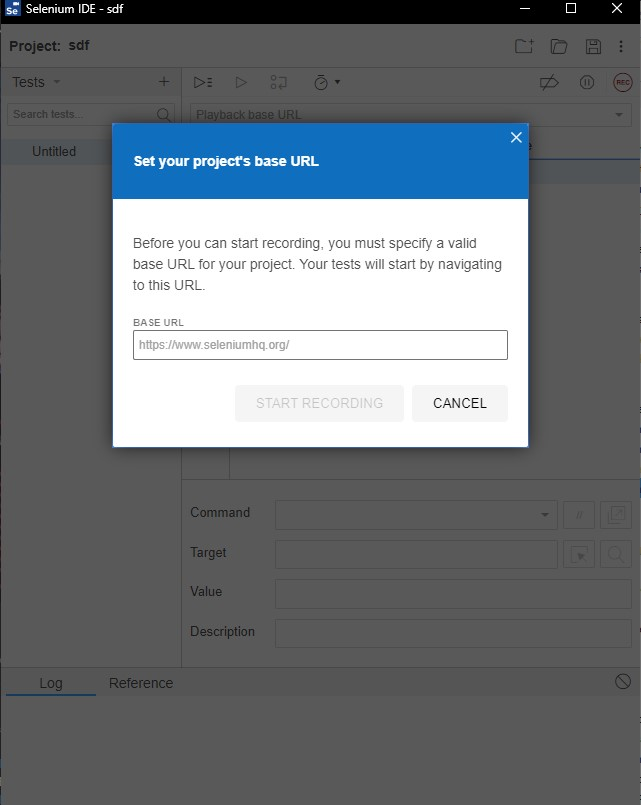
\includegraphics[scale=0.4]{Gambar/baseURL.jpg}
			\caption{Tampilan Memasukan Situs Web} 
			\label{fig:baseURL}
		\end{figure}
		Setelah menekan tombol ``\textit{START RECORDING}'' seperti pada Gambar \ref{fig:baseURL}, maka akan langsung muncul \textit{windows} Google Chrome baru yang langsung menuju situs web yang sudah dimasukan tadi.
		\item Melakukan apa yang ingin diotomatisasikan di \textit{windows} Google Chrome baru yang sudah menuju situs web hingga selesai dan menutup \textit{windows} Google Chrome.
		\begin{figure}[H]
			\centering
			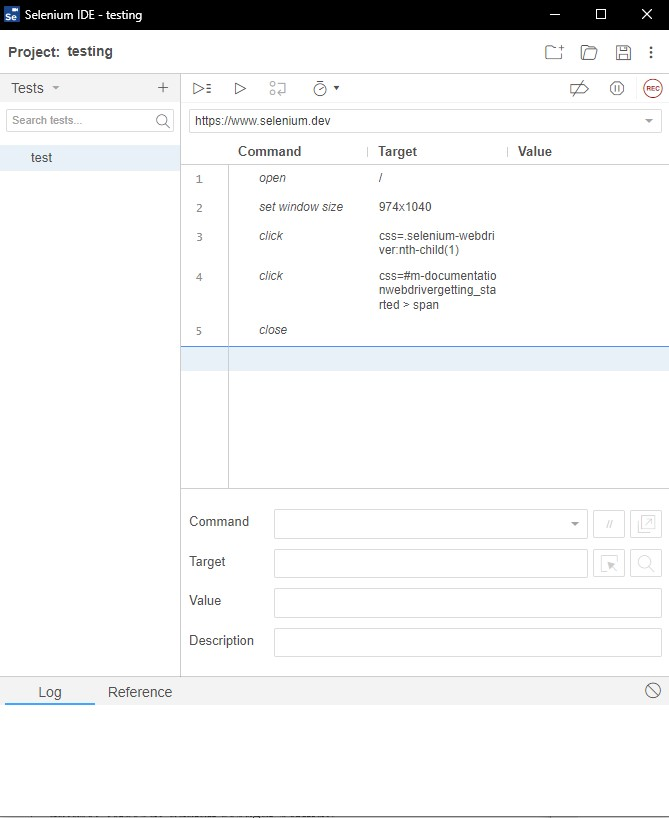
\includegraphics[scale=0.4]{Gambar/testing.jpg}
			\caption{Tampilan Otomatisasi pada Selenium IDE} 
			\label{fig:testing}
		\end{figure}
		Pada Gambar \ref{fig:testing} menunjukan hasil yang sudah terekam dari apa yang sudah dilakukan pada situs web yang ingin diotomatisasikan.
	\end{enumerate}